\documentclass[a4paper,10pt, leqno]{article}
\usepackage[utf8]{inputenc}
\usepackage{mathtools}
\usepackage{amsfonts}
\usepackage{amssymb}
\usepackage{amsthm}
\usepackage{graphicx}
\usepackage{indentfirst}
\usepackage{array}
\usepackage{bm}

\def\blankpage{%
      \null%
      \clearpage}

\let\oldref\ref
\renewcommand{\ref}[1]{(\oldref{#1})}

%opening
\title{MAC0325 Combinatorial Optimization \\
        \large Assignment 1 }
\author{Pedrog Gigeck Freire \\
        10737136}
\date{October 06, 2020}

%\setlength{\parindent}{0.5em}
%\setlength{\parskip}{0.1em}
\begin{document}

\maketitle

\section*{Exercise 6}
Given a digraph $D = (V, A, \varphi)$ and a cost 
function  $c : A \to \mathbb{R}$ and $r, s \in V$.

We adopt the notation $v_i = (v, i)$ for $v \in V$, $i \in \mathbb{Z}$.

Let $D' \coloneqq (V', A', \varphi')$ be a digraph with 
$$V' \coloneqq V \times \{0, 1\} $$
$$A' \coloneqq A \times \{0, 1\} $$
$$\varphi' : A' \to V' \times V' \text{ given by}$$
$$\varphi'((a, i)) \coloneqq
\left\{
	\begin{array}{ll}
		(u_0, w_1)  & \mbox{if } i = 0 \text{, where } \varphi(a) = (u, w) \\
		(u_1, w_0)  & \mbox{if } i = 1 \text{, where } \varphi(a) = (u, w) \\
	\end{array}
\right.$$

Figure \ref{fig:graph1} is an example of $D'$ obtained from an original digraph $D$.

\begin{figure}[h]
\centering
  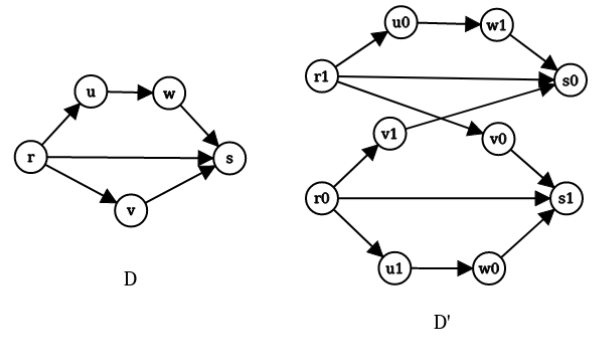
\includegraphics[width=30em]{graph.png}
  \caption{Example of transformation from $D$ to $D'$.}
  \label{fig:graph1}
\end{figure}

Let $c' : A' \to \mathbb{R}$ be a cost function given by
$c'((a, i)) \coloneqq c(a)$.

We define the following instance of the shortest walk problem:

\begin{equation}
\tag{6.2}\label{swp}
    \begin{aligned}
    & \text{Minimize}
    & & c'(W) \\
    & \text{subject to}
    & & W \text{ is an $(r_0, s_0)$-walk in } D' 
    \end{aligned}
\end{equation} 

We claim that problem \ref{swp} and problem (6.1) (given in the exercise) are homomorphically equivalent.

To prove it, we need to define some notation:

Let $W_2(D)$ be the set of all walks in $D$ that have even length.

Let $V'_0 \coloneqq \{(v, 0), v \in V \}$ be a subset of $V'$.

Let $W_0(D') \coloneqq \{ (u_0, w_0)\text{-walks in } D' : u_0, w_0 \in V'_0\}$ be the set of all walks in $D'$ that starts in $V'_0$ and ends in $V'_0$. 

Let $X$ be the set of feasible solutions of problem (6.1), i.e., the set of $(r, s)$-walks in $D$ that have even length.

Let $Y$ be the set of feasible solutions of problem \ref{swp}, i.e., the set of $(r_0, s_0)$-walks in $D'$. 

From now on, $v_i$ denotes the vertices of $V$ and $(v_i, j)$ denotes de vertices of $V'$. 

Let $\xi : W_2(D) \to W_0(D')'$ be a function defined recursively by:

Given $W \coloneqq \langle v_0, a_1, v_1, ..., a_l, v_l\rangle \in W_2(D)$, 
\begin{align*}
\xi(\langle v_0 \rangle) &\coloneqq \langle (v_0, 0) \rangle & & & & & \text{if } l = 0 \\
\xi(\langle v_0, a_1, v_1, a_2, v_2\rangle) &\coloneqq  \langle (v_0, 0), (a_1, 0), (v_1, 1), (a_2, 1), (v_2, 0) \rangle & & & & & \text{if } l = 2 \\
\xi(\langle v_0, a_1, v_1, ..., a_l, v_l\rangle) &\coloneqq \xi(\langle v_0, ..., v_2 \rangle) \cdotp \xi(\langle v_2, ..., v_l\rangle & & & & & \text{if } l > 2
\end{align*}

It is simple to verify by induction that if $W \in W_2(D)$ is a $(u, w)$-walk in $D$ then $\xi(W)$ is a $(u_0, w_0)$-walk in $D'$, so $\xi(W) \in W_0(D')$ and the function $\xi$ is, indeed, a (well defined) function. 

Let $\phi : X \to Y$ be a function given by $\phi(W) \coloneqq \xi(W)$ 

\newtheorem{lemma}{Lemma}
\begin{lemma}
    \label{homo1}
    $\phi$ is a homomorphism from (6.1) to \ref{swp}. 
\end{lemma}
\begin{proof}
    Given $W \in X$, the length of $W$ is equal to the length of $\phi(W)$, and the arcs in both walks have the same costs.
    Formally,
    \begin{align*}c'(\phi(W)) &= \sum_{(a, i) \in A(\phi(W))}{c'((a, i))}  \\
    &= \sum_{a \in A(W)}{c(a)} 
    = c(W) \\
    \end{align*}
    
    So $W \in L_{(6.1)}(\mu) \implies c(W) \leq \mu \implies c'(\phi(W)) \leq \mu$.
    
    Then $\phi(W) \in L_{(6.2)}(\mu)$. So $\phi$ is a homomorphism .
\end{proof}

\newtheorem{proposition}[lemma]{Proposition}
\begin{proposition} \label{prop1}
    Every walk $W \in W_0(D')$ has even length.
\end{proposition}
\begin{proof}
Let $W \in W_0(D')$, let $l$ be the length of $W$.
We prove by induction on $l$.
   
If $l = 0$, then $l$ is even.

There is no walk in $W_0(D')$ of length 1, because every arc with origin in $V'_0$ ends in an arc of the form $(v, 1)$, by the definition of the incidence function $\varphi'$.
   
Suppose that $l \geq 2$, and every walk $W' \in W_0(D')$ of length $l' < l$ has even length ($l'$ is even). 

Let $W = \langle (v_0, 0), (a_1, 0), (v_1, 1), (a_2, 1), (v_2, 0) ..., (a_l, 1), (v_l, 0) \rangle$. Suppose by the sake of contradiction that $l$ is odd. Let $ W' \coloneqq \langle (v_2, 0), ..., (a_l, 1), (v_l, 0) \rangle$, then $W'$ has odd length $l' = l - 2$, but $l' < l$ and $W' \in W_0(D')$, contradiction.
    
\end{proof}


Let $\chi : W_0(D') \to W_2(D)$ be a function defined by, given $W' \in W_0(D')$ with length $l$: 
\begin{align*}
\chi(\langle (v_0, 0) \rangle) \coloneqq& \langle v_0 \rangle & & & & & \text{if } l = 0 \\
\chi(\langle (v_0, 0), (a_1, 0), (v_1, 1), (a_2, 1), (v_2, 0) \rangle) \coloneqq& \langle v_0, a_1, v_1, a_2, v_2\rangle  & & & & & \text{if } l = 2 \\
\chi(\langle (v_0, 0), (a_1, 1), (v_1, 1), ..., (a_l, 1), (v_l, 0)\rangle) \coloneqq& \chi(\langle (v_0, 0), ..., (v_2, 0) \rangle) \cdotp \\ & \chi(\langle (v_2, 0), ..., (v_l, 0)\rangle & & & & & \text{if } l > 2
\end{align*}

We can notice that $\chi$ is well defined directly from proposition \ref{prop1} (every walk in $W_0(D')$ has even length).

Let $\psi : Y \to X$ be a function given by $\psi(W') \coloneqq \chi(W')$ 
\begin{lemma}
    \label{homo2}
    $\psi$ is a homomorphism from \ref{swp} to (6.1). 
\end{lemma}
\begin{proof}
    Given $W' \in Y$, the length of $W'$ is equal to the length of $\psi(W')$, and the arcs in both walks have the same costs.
    Formally,
    \begin{align*}c(\psi(W')) &= \sum_{a \in A(\psi(W'))}{c(a)}  \\
    &= \sum_{(a, i) \in A(W')}{c'(a, i)}
    = c'(W') \\
    \end{align*}
    
    So $W' \in L_{(6.2)}(\mu) \implies c'(W') \leq \mu \implies c(\psi(W')) \leq \mu$.
    
    Thus $\psi(W') \in L_{(6.1)}(\mu)$. So $\psi$ is a homomorphism.
\end{proof}

\newtheorem{theorem}{Theorem}
\begin{theorem}
    Problems (6.1) and \ref{swp} are homomorphically equivalent. 
\end{theorem}
\begin{proof}
    Imediate from lemmas \ref{homo1} and \ref{homo2}
\end{proof}

\section*{Exercise 9}

We will write a compact proof that needs to be read carefully in both directions. Each step comes straightforward from definitions.

For each $x \in X$, take $\mu \coloneqq f(x)$.
\begin{align*}
\varphi \text{ homomorphism } &\implies \varphi(L_\mathcal{O}(\mu)) \subseteq L_\mathcal{P}(\mu)\\
& \iff \varphi(\{x \in X : \alpha f(x) \geq \alpha \mu \}) \subseteq L_\mathcal{P}(\mu) \\
& \iff \varphi(\{x \in X : \alpha f(x) \geq \alpha f(x) \}) \subseteq L_\mathcal{P}(\mu) \\
& \iff \varphi(X) \subseteq L_\mathcal{P}(\mu) \\
& \iff \varphi(X) \subseteq L_\mathcal{P}(f(x)) \\
& \iff \varphi(X) \subseteq \{ y \in Y : \alpha g(y) \geq \alpha f(x)\}\\
& \iff \varphi(x) \in \{ y \in Y : \alpha g(y) \geq \alpha f(x)\} \text{, } \forall x \in X \\
& \iff \alpha g(\varphi(x)) \geq \alpha f(x) \text{, } \forall x \in X 
\end{align*}

The only step that is not straightforward is the way back of the first implication.

We have that 
$\varphi(L_\mathcal{O}(\mu)) \subseteq L_\mathcal{P}(\mu)$
for every $\mu$ of the form $\mu = f(x)$ but not for every $\mu \in \mathbb{R}$.

But we claim thar being valid in the range of $f$ is sufficient to be valid in the whole real set. 
Let $\nu \in \mathbb{R}$ be any real number, so $L_\mathcal{O}(\nu) = \{x \in X : \alpha f(x) \geq \alpha \nu \}$. So every element in $L_\mathcal{O}(\nu)$ has a value in $f$ greater or equal than some other value. We may take the greatest value of these, say $f(x*)$ and $L_\mathcal{O}(\nu) \subseteq L_\mathcal{O}(f(x*))$

Thus $\varphi$ will be, indeed, a homomorphism.

\blankpage

\section*{Exercise 12}

In each iteration of the \textbf{for} loop, we list the matching $\bf{M_t}$ that is already defined in the beggining of the iteration and the augmenting path found in the end of the iteration (this path generates the next matching $M_{t + 1}$) 

\bgroup
\def\arraystretch{1.8}
\begin{center}
\begin{tabular}{|m{0.4cm}|m{9cm}|m{2cm}|}
\hline
\centering $\bm{t}$ & \centering{$\bm{M_t}$} & \textbf{Augmenting Path found}\\
\hline
\centering $0$ & $\emptyset$ & $\langle a, A \rangle$ \\
\hline
\centering $1$ & $\{ (a, A) \}$ & $\langle b, B \rangle$ \\
\hline
\centering $2$ & $\{ (a, A), (b, B)\}$ & $\langle c, D \rangle$ \\
\hline
\centering $3$ & $\{ (a, A), (b, B), (c, D) \}$ & $\langle f, C \rangle$ \\
\hline
\centering $4$ & $\{ (a, A), (b, B), (c, D), (f, C) \}$ & $\langle g, E \rangle$ \\
\hline
\centering $5$ & $\{ (a, A), (b, B), (c, D), (f, C), (g, E) \}$ & $\langle h, F \rangle$ \\
\hline
\centering $6$ & $\{ (a, A), (b, B), (c, D), (f, C), (g, E), (h, F) \}$ & $\langle i, I \rangle$ \\
\hline
\centering $7$ & $\{ (a, A), (b, B), (c, D), (f, C), (g, E), (h, F), (i, I) \}$ & $\langle d, A, a, B, $ \newline $ b, C, f, H \rangle$ \\
\hline
\centering $8$ & $\{ (a, B), (b, C), (c, D), (d, A), (f, H), (g, E), (h, F), (i, I) \}$ & - \\
\hline
\end{tabular}
\end{center}
\egroup

In the end of algorithm, the vertex cover found is the set $\{b, f, g, h, A, B, D, I \}$

\blankpage
\blankpage

\section*{Exercise 13}

Let $G$ be a $(U, W)$-bipartite graph

\begin{lemma}[$(i) \implies \neg{(ii)}$]
If $G$ has a matching that saturates U, then $|S| \leq |N(S)|$ for each $S \subseteq U$.
\end{lemma}
\begin{proof}
Let $M$ be a matching in $G$ that saturates $U$.
For each $s \in S$ there is an edge $e \in M$ that connects $s$ with one unique $w \in W$. So there are at least $|S|$ vertices in $N(S)$.
\end{proof}

\begin{lemma}[$\neg{(i)} \implies (ii)$]
If no matching in $G$ saturates U, then there is a subset $S \subseteq U$ such that $|S| > |N(S)|$.
\end{lemma}
\begin{proof}
Let $M$ be a maximum matching in $G$. By hyposthesis, there are vertices in $U$ that are not saturated by $M$.

Let $R \coloneqq\{ v \in V : \text{ there is } u \in U \setminus V_M \text{
such that } u \rightsquigarrow
v\}$ be the set (defined in the algorithm) of vertices reacheable from unsaturated vertices in $U$.

Let $S \coloneqq U \cap R$. We have that $N(S) \subset (R \cap W)$, by definition of R (the reacheable vertices)  

Since $M$ is maximum, the algorithm correctness implies that every vertice in $N(S)$ is saturates , because if there was one unsaturated, there would be an augmenting path and $M$ would not be maximum.

So, for every vertice in $N(S)$ there is one unique vertice in $(S \cap V_M$ (the other end of the matching edge). From this we get that $|S \cap V_M| = |N(S)|$.

But there is at least one vertice in S that is not in $S \cap V_M$. Therefore $|S| > |S \cap V_M| = |N(S)|$.
\end{proof}

From the law of excluded middle. We may divide our exercise in two cases:

Case 1: $(i)$ holds.
From lemma 4, we have that $(ii)$ fails, thus exactly one of the options holds.

Case 2: $(i)$ fails.
From lemma 5, we have that $(ii)$ holds, thus exactly one of the options holds.



\end{document}

